\chapter{Closed Section A}
\label{ch:assignment1}



\bigskip
\tbd{Inleiding van dit hoofdstuk: beschrijving van sectie~A (machinekamer),
de buitenrand en de binnenrand (schaalfactor $k$), de gebruikte
Prandtl-spanningsfunctie $\phi(y,z)$ en de aannames die hier gelden.}

\section{Location of maximum shear stress}
\label{sec:a1-1}
The given Prandtl stress function shows the stress in the section with the use of isolines and gradients of said isolines. The steepnes of this gradient is given by the density of these isolines. In this case the lines are closest in Z direction at the top of the section at (0,1) and closest in Y direction on (1,0) \& (0,1). Therefore the shear stress is maximum at these points for their respective direction.

\begin{figure}[h]
    \centering
    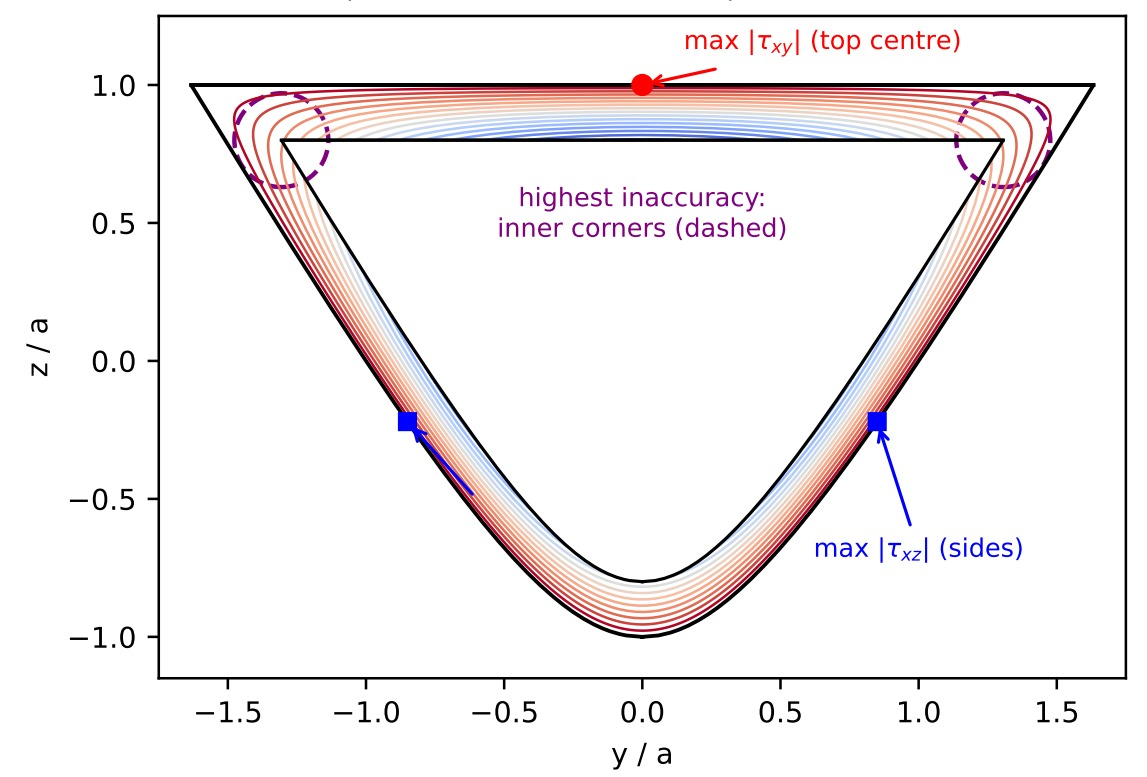
\includegraphics[width=0.95\linewidth]{figures/A1_prandtl (2).jpeg}
    \caption{Areas of highest inaccuracy}
    \label{fig: prandtl}
\end{figure}

\noindent\textbf{Final answer.} $|\tau_{xy}|$ is maximal at the middle of the top plate. $|\tau_{xz}|$ is maximal on the two inclined side walls just below the $y$-axis.

\section{Inaccuracies of the Prandtl-based prediction}
\label{sec:a1-2}


For a hollow section, the solid-section stress function only gives the exact solution if the inner boundary happens to lie exactly on one of its contour lines (i.e. $\phi$ is constant along it). Figure \ref{fig: prandtl} shows that this is not the case here: the scaled inner boundary cuts across several isolines instead of following one, especially near the inner top corners and the upper part of the inclined walls (dashed in the figure). Because of this, two things go wrong. First, the predicted shear stress on the inner wall is not fully tangential to the boundary, so part of it points through the free surface, which cannot actually happen. Second, the magnitude is off: a thin hollow wall should carry a roughly constant shear flow around it, while the solid-section solution predicts a stress that varies a lot from point to point. As a result, the torque-twist relation derived from this stress function is also only approximate. The prediction is closest to reality at the centre of the top wall and at the bottom, since the boundary there runs almost parallel to a contour line.

\noindent\textbf{Final answer.} The Prandtlbased prediction breaks the tractionfree condition on the inner wall and gets the shearflow magnitude wrong. The error is largest at the inner top corners and the adjacent inclined walls (dashed in Figure \ref{fig: prandtl}), and smallest at the centre of the top wall and at the bottom


\section{Cross-sectional efficiency}
\label{sec:a1-3}

\subsection{Areas.}
The inner boundary is a copy of the outer boundary, scaled by $k$. All lengths scale by $k$, so every area scales by $k^2$:
\begin{equation}
    A_{inner} = k^2 A_{solid}
\end{equation}
The hollow section is the solid section minus the hole:
\begin{equation}
    A_{hollow} = A_{solid} - A_{inner} = (1-k^2)\,A_{solid}
\end{equation}

\subsection{Torsional constant of the inner section.}
From the lectures, the torsional constant follows from the Prandtl stress function:
\begin{equation}
    I_p = \frac{M_t}{G\theta'} = \frac{2}{G\theta'}\int_A \phi \, dA
    \label{eq:a1-Ip}
\end{equation}
where $\phi$ satisfies the Poisson equation, with $\phi = 0$ on the boundary:
\begin{equation}
    \frac{\partial^2\phi}{\partial y^2} + \frac{\partial^2\phi}{\partial z^2} = -2G\theta'
    \label{eq:a1-poisson}
\end{equation}
Now we treat the inner section as a solid section on its own. Every point of it is a scaled point of the solid section, $y = k\hat{y}$ and $z = k\hat{z}$, where $(\hat{y},\hat{z})$ runs over the solid section. By the chain rule, each derivative gives a factor $1/k$:
\begin{equation}
    \frac{\partial^2\phi_{inner}}{\partial y^2} = \frac{1}{k^2}\,\frac{\partial^2\phi_{inner}}{\partial \hat{y}^2},
    \qquad
    \frac{\partial^2\phi_{inner}}{\partial z^2} = \frac{1}{k^2}\,\frac{\partial^2\phi_{inner}}{\partial \hat{z}^2}
\end{equation}
Substituting this into Eq.~\eqref{eq:a1-poisson} gives
\begin{equation}
    \frac{\partial^2(\phi_{inner}/k^2)}{\partial \hat{y}^2} + \frac{\partial^2(\phi_{inner}/k^2)}{\partial \hat{z}^2} = -2G\theta'
\end{equation}
So $\phi_{inner}/k^2$ satisfies exactly the same equation as $\phi_{solid}$, on the same shape and with the same boundary condition ($=0$ on the edge). It must therefore be the same function:
\begin{equation}
    \phi_{inner}(y,z) = k^2\,\phi_{solid}(\hat{y},\hat{z})
\end{equation}
The area element scales as $dA = k^2\,d\hat{A}$. Putting both into Eq.~\eqref{eq:a1-Ip}:
\begin{equation}
    I_{p,inner} = \frac{2}{G\theta'}\int_{A_{solid}} k^2\phi_{solid}\;k^2\,d\hat{A}
    = k^4\,\frac{2}{G\theta'}\int_{A_{solid}} \phi_{solid}\,d\hat{A}
    = k^4\,I_{p,solid}
\end{equation}
As a check: for a circle $I_p = \pi R^4/2$, so a radius $kR$ gives exactly a factor $k^4$.

\subsection{Torsional constant of the hollow section.}
Removing the core removes its contribution to the stiffness. This is exact only when the inner boundary lies on a contour line of $\phi_{solid}$ (e.g.\ a circle or ellipse). Question~\ref{sec:a1-2} showed this is not the case here, so it is an approximation:
\begin{equation}
    I_{p,hollow} \approx I_{p,solid} - I_{p,inner} = (1-k^4)\,I_{p,solid}
\end{equation}

\subsection{Cross-sectional efficiency.}
\begin{equation}
    \eta(k) = \frac{I_{p,hollow}/A_{hollow}}{I_{p,solid}/A_{solid}}
    = \frac{1-k^4}{1-k^2}
    = \frac{(1-k^2)(1+k^2)}{1-k^2}
    = 1+k^2
\end{equation}
This is plotted in Figure~\ref{fig:efficiency}, together with the relative area $(1-k^2)$ and the relative stiffness and strength $(1-k^4)$.

\begin{figure}[h]
    \centering
    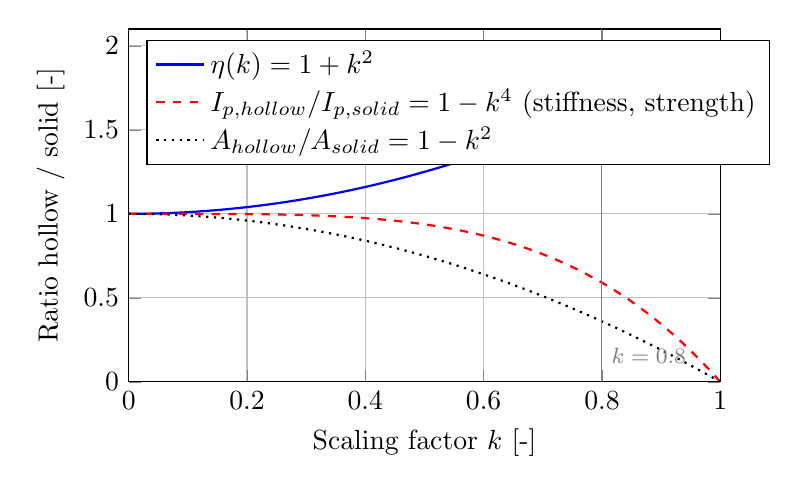
\begin{tikzpicture}
        \begin{axis}[
            width=0.75\textwidth,
            height=0.5\textwidth,
            xlabel={Scaling factor $k$ [-]},
            ylabel={Ratio hollow / solid [-]},
            xmin=0, xmax=1,
            ymin=0, ymax=2.1,
            grid=major,
            legend pos=north west,
            legend cell align=left,
            domain=0:1,
            samples=100,
        ]
            \addplot[thick, blue] {1 + x^2};
            \addlegendentry{$\eta(k) = 1+k^2$}
            \addplot[thick, red, dashed] {1 - x^4};
            \addlegendentry{$I_{p,hollow}/I_{p,solid} = 1-k^4$ (stiffness, strength)}
            \addplot[thick, black, dotted] {1 - x^2};
            \addlegendentry{$A_{hollow}/A_{solid} = 1-k^2$}
            % example point k = 0.8
            \draw[gray, thin] (axis cs:0.8,0) -- (axis cs:0.8,2.1);
            \node[gray, anchor=south west, font=\footnotesize] at (axis cs:0.8,0.05) {$k=0.8$};
        \end{axis}
    \end{tikzpicture}
    \caption{Cross-sectional efficiency $\eta(k) = 1+k^2$ and the relative torsional stiffness, strength and area of the hollow section as a function of the scaling factor $k$.}
    \label{fig:efficiency}
\end{figure}

\subsection{Efficiency versus strength.}
Strength here means the largest torque the section can carry before the maximum shear stress reaches the allowable value. Within the same approximation, the stresses in the remaining material are the same as in the solid section at the same twist rate, so $\tau_{max}$ stays on the unchanged outer boundary:
\begin{equation}
    \tau_{max,hollow}(\theta') = \tau_{max,solid}(\theta')
\end{equation}
For the same torque, however, the hollow section twists more:
\begin{equation}
    \theta'_{hollow} = \frac{M_t}{G I_{p,hollow}} = \frac{\theta'_{solid}}{1-k^4}
\end{equation}
Since Eq.~\eqref{eq:a1-poisson} is linear in $G\theta'$, $\phi$ and therefore $\tau_{max}$ are proportional to $\theta'$. This gives
\begin{equation}
    \tau_{max,hollow} = \frac{\tau_{max,solid}}{1-k^4}
    \quad\Rightarrow\quad
    M_{t,max,hollow} = (1-k^4)\,M_{t,max,solid}
\end{equation}

So the efficiency rises from 1 (solid, $k=0$) to 2 ($k\to1$), because the removed core carried little stress, but the absolute stiffness and strength both drop with $(1-k^4)$. For $k=0.8$ the section uses 36\% of the material and $\eta = 1.64$, but it only carries 59\% of the torque of the solid section. Past $k\approx0.9$ there is little left to gain in $\eta$ (it is capped at 2), while $(1-k^4)$ keeps dropping fast. On top of that, the approximation from Question~\ref{sec:a1-2} gets worse for thin walls: it misses the stress concentrations at the inner corners, and very thin walls can also buckle in shear. A moderate $k$ is therefore the best balance: hollow enough to save real material, but not so thin that the strength collapses.

\subsection{Final answer.} $A_{inner}=k^2A_{solid}$, $A_{hollow}=(1-k^2)A_{solid}$, $I_{p,inner}=k^4I_{p,solid}$, $I_{p,hollow}\approx(1-k^4)I_{p,solid}$, $\eta(k)=1+k^2$ (Figure~\ref{fig:efficiency}).



